\documentclass[russian,aspectratio=169,14pt]{beamer}

\usetheme{ShipilevRH}

\title{Работа с базами данных}
\subtitle{JDBC}
\author{Валерий Алексеевич Овчинников}
\institute{valery.ovchinnikov@phystech.edu}

\begin{document}

\maketitle

\section{Мотивация}

\begin{frame}
	\begin{itemize}
		\item Практически любое серьезное приложение что-то хранит (данные, конфигурацию, состояние)
		\pause
		\item Самым распространенным способом хранить данные является использование реляционных баз данных
		\pause
		\item При работе с RDBMS из Java прямо или опосредованно исползуется JDBC
	\end{itemize}
\end{frame}

\section{JDBC}

\begin{frame}
	\frametitle{Architecture}
	\begin{center}
	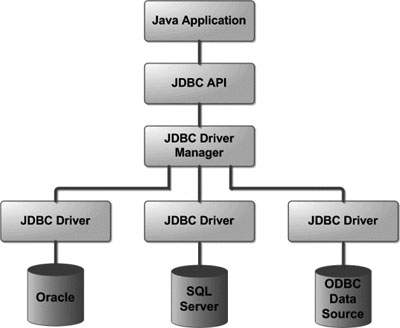
\includegraphics[height=0.75\textheight]{jdbc-architecture.jpg}
	\end{center}
\end{frame}

\begin{frame}
	\frametitle{Driver}
	Существует 4 типа JDBC драйверов:
	\vfill
	\begin{enumerate}
		\item JDBC-ODBC мост (является адаптером к ODBC драйверу)
		\item JDBC - Native API (использует нативные вызовы в базу)
		\item JDBC-Net pure Java (использует сервер-посредник)
		\item 100\% pure Java (предпочтительный)
	\end{enumerate}
\end{frame}

\begin{frame}
	\frametitle{Driver}
	Нужно узнать имя драйвера для вашей RDBMS
	\vfill
	\begin{center}
	\begin{tabular}{l|l}
		\small
		RDBMS & Driver name \\
		\hline
		\hline
		\texttt{MySQL} & \texttt{com.mysql.jdbc.Driver} \\
		\hline
		\texttt{Oracle} & \texttt{oracle.jdbc.driver.OracleDriver} \\
		\hline
		\texttt{DB2} & \texttt{COM.ibm.db2.jdbc.net.DB2Driver} \\
		\hline
		\texttt{Sybase} & \texttt{com.sybase.jdbc.SybDriver} \\
		\hline
		\texttt{PostgreSQL} & \texttt{org.postgresql.Driver} \\
		\hline
	\end{tabular}
	\end{center}
\end{frame}

\begin{frame}[fragile]
	\frametitle{Driver}
	Драйвер нужно зарегестрировать (достаточно загрузить класс)
	\begin{listjava}
Class.forName(DB_DRIVER);
	\end{listjava}
\end{frame}

\begin{frame}
	\frametitle{Connection}
	Для подключения к базе нужно составить jdbc-url
	\vfill
	\begin{center}
	\begin{tabular}{l|l}
		\small
		RDBMS & URL format \\
		\hline
		\hline
		\texttt{MySQL} & \texttt{jdbc:mysql://hostname/database} \\
		\hline
		\texttt{Oracle} & \texttt{jdbc:oracle:thin:@hostname:port:databaseName}	\\
		\hline
		\texttt{DB2} & \texttt{jdbc:db2:hostname:port/databaseName} \\
		\hline
		\texttt{Sybase} & \texttt{jdbc:sybase:Tds:hostname:port/database} \\
		\hline
		\texttt{PostgreSQL} & \texttt{jdbc:postgresql://host:port/database} \\
		\hline
	\end{tabular}
	\end{center}
\end{frame}

\begin{frame}[fragile]
	\frametitle{Connection}
	\begin{listjava}
try (Connection conn = DriverManager.getConnection(String url)) {}
Connection conn = DriverManager
        .getConnection(String url, Properties prop);
Connection conn = DriverManager
        .getConnection(String url, String user, String password);
	\end{listjava}
\end{frame}

\begin{frame}
	\frametitle{Statements}
	Существует 3 типа Statement:
	\vfill
	\begin{enumerate}
		\item Statement -- для выполнения статических SQL выражений
		\item PreparedStatement -- для SQL выражений с параметрами (рекомендуются, переиспользуемые)
		\item CallableStatement -- для вызова хранимых (в базе) процедур
	\end{enumerate}
\end{frame}

\begin{frame}[fragile]
	\frametitle{Statement}
	\begin{listjava}
try (Statement st = conn.createStatement()) {
	boolean st.execute(String sql);
	int st.executeUpdate(String sql); // insert, update, delete
	ResultSet st.executeQuery(String sql); // select
}
	\end{listjava}
\end{frame}

\begin{frame}[fragile]
	\frametitle{PreparedStatement}
	\begin{listjava}
try (PreparedStatement st = conn.prepareStatement(sql)) {
	boolean st.execute(String sql);
	int st.executeUpdate(String sql);
	ResultSet st.executeQuery(String sql);
}
	\end{listjava}
\end{frame}

\begin{frame}[fragile]
	\frametitle{Transactions}
	По умолчанию включен autocommit
	\vfill
	\begin{listjava}
conn.setAutoCommit(false);
conn.commit();
conn.rollback();
	\end{listjava}
\end{frame}

\begin{frame}[fragile]
	\frametitle{Transactions}
	\begin{listjava}
Savepoint savepoint = conn.setSavepoint("Savepoint1");
try {
    stmt.executeUpdate(SQL1);
    stmt.executeUpdate(SQL2);
} catch(SQLException e) {
	conn.rollbacl(savepoint);
}
	\end{listjava}
\end{frame}

\begin{frame}[fragile]
	\frametitle{Batch updates}
	Если нужно выполнить несколько команд, то эффективнее использовать batching
	\begin{listjava}
conn.setAutoCommit(false);
st.addBatch(sql1);
st.addBatch(sql2);
st.executeBatch();
	\end{listjava}
\end{frame}


\begin{frame}[fragile]
	\frametitle{JOOQ}
	Существуют обертки над JDBC (e.g. Spring JDBCTemplated, JOOQ)\\
	JOOQ:
	\begin{listjava}
DSLContext create = DSL.using(conn, SQLDialect.POSTGRES);
Result<Record> result = create.select().from(AUTHOR).fetch();
for (Record r : result) {
    Integer id = r.getValue(AUTHOR.ID);
    String firstName = r.getValue(AUTHOR.FIRST_NAME);
    String lastName = r.getValue(AUTHOR.LAST_NAME);
    
    System.out.println("ID: " + id + " first name: " +
         firstName + " last name: " + lastName);
}
	\end{listjava}
\end{frame}


\questions

\end{document}
